%%%%%%%%%%%%%%%%%%%%%%%%%%%%%%%%%%%%%%%%%%%%%%%%%%%%%%%%%%%%%%%%%%%%%%
%%%%%%%%%%%%%%%%%%%%%%%%%%%%%%%%%%%%%%%%%%%%%%%%%%%%%%%%%%%%%%%%%%%%%%
\documentclass[dvips]{seminar}                      %%%%%%%%%%%%%%%%%%
                                                    %%%%%%%%%%%%%%%%%%
%  make KKres-ps
%  make KKres-pdf

%%%%%%%%%%%%%%%%%%%%%%%%%%%%%%%%%%%%%%%%%%%%%%%%%%%%%%%
%%%%%%%%%%%%%%%%%%%%%%%%%%%%%%%%%%%%%%%%%%%%%%%%%%%%%%%
\begin{document}                     %%%%%%%%%%%%%%%%%%


% The upper title is defined in seminar.con One may redefine it like that
\def\title{{\large KKMC and RRes for low energy colliders}}


%//////////////////////////////////////////////////////////////////////////////////
%//////////////////////////////////////////////////////////////////////////////////
\begin{slide}

\begin{center}
{\LARGE\bf\crd   KKMC and RRes for low energy colliders}\\
\vspace{2mm}
{\LARGE\bf\cbl   S. Jadach}\\
\vspace{2mm}
{\large\bf       Institute of Nuclear Physics, Krak\'ow, Poland}
\end{center}
%===================================================================

\vspace{10mm}
{\small\Cmar
  Outline:
  \begin{itemize}
  \item
    ...
  \item
    ...
  \end{itemize}
}

{\cbl\small\bf KKMC available from  http://home.cern.ch/jadach}
\vfill
\end{slide}   %%%
%%%%%%%%%%%%%%%%%%

%//////////////////////////////////////////////////////////////////////////////////
%//////////////////////////////////////////////////////////////////////////////////
%//////////////////////////////////////////////////////////////////////////////////
\begin{slide}
\yellowbox{\crd\bf RRes package of M. Boonekamp, now included in \KK MC}
{\cbl
  \begin{itemize}
  \item
    $R(s)$ from most available hadronic data, old ones (SLAC, Orsay)
    and new (Novosibirsk).
  \item
    In particular $\rho$ and $\omega$ region parametrized using new Novosibirsk data,
    hep-ex/9904027.
  \item
    In MC generation $R(s)$ split into resonant and non-resonant parts.
    $R(s)$ is also split among available  $q_i\bar{q}_i$ pairs, for resonances and continuum.
  \item
    Resonance decays (from $\rho$ to $\Upsilon$) generated using Pythia tool.
  \item
    Non-resonant  ``continuum'' part modelled using Pythia tool for $q_i\bar{q}_i$ string.
    At $\sqrt{s}<2GeV$ for (small) non-resonant component flat phase space is used
    experimental data are used to determine the type of final state (any channel).
  \item
    No naive QCD applied for ``continuum'', for the moment.
  \end{itemize}
}
To be improved: for continuum part replace flat phase space
with more realistic description of $n\pi$ state,
better matching with perturbative QCD and QED (FSR).

\vfill
\end{slide}    %%%
%%%%%%%%%%%%%%%%%%



%//////////////////////////////////////////////////////////////////////////////////
%//////////////////////////////////////////////////////////////////////////////////
%//////////////////////////////////////////////////////////////////////////////////
\begin{slide}
\yellowbox{\bf\crd\Large  $q\bar{q}$ SKYLINE from RRes package}
\vspace{-3mm}
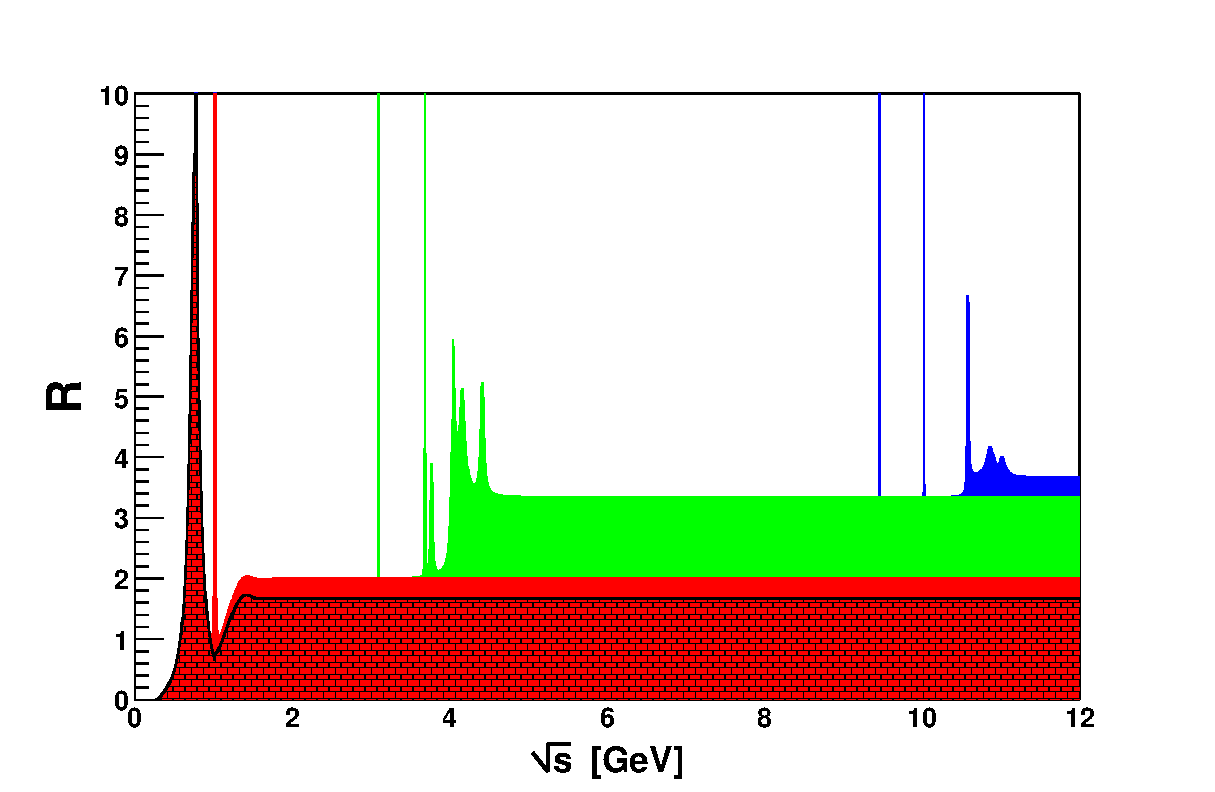
\epsfig{file=../Plots/cRtot.eps,width=120mm}

\vfill
\end{slide}    %%%
%%%%%%%%%%%%%%%%%%



%//////////////////////////////////////////////////////////////////////////////////
%//////////////////////////////////////////////////////////////////////////////////
%//////////////////////////////////////////////////////////////////////////////////
\begin{slide}
\yellowbox{\bf\crd  Zoom on resonances  (RRes package)}

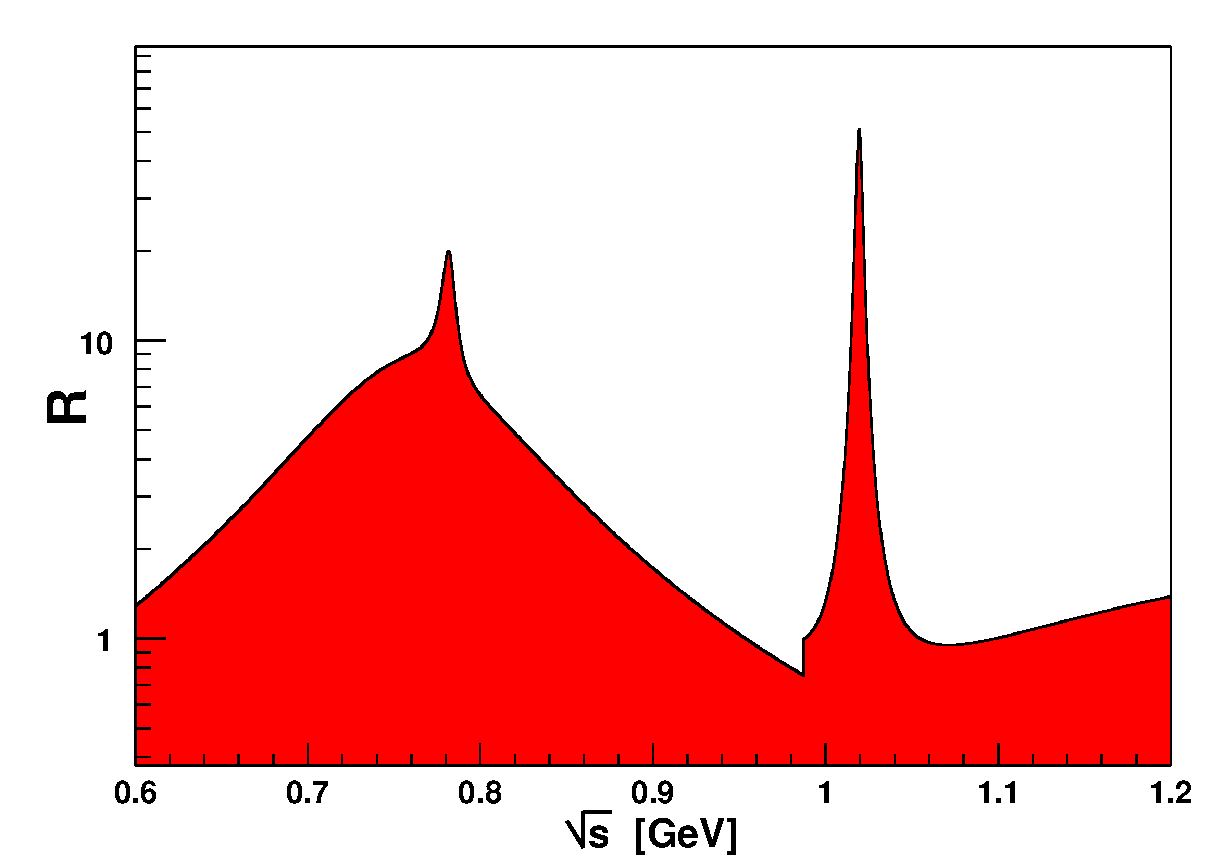
\epsfig{file=cRrho.eps,width=52mm}
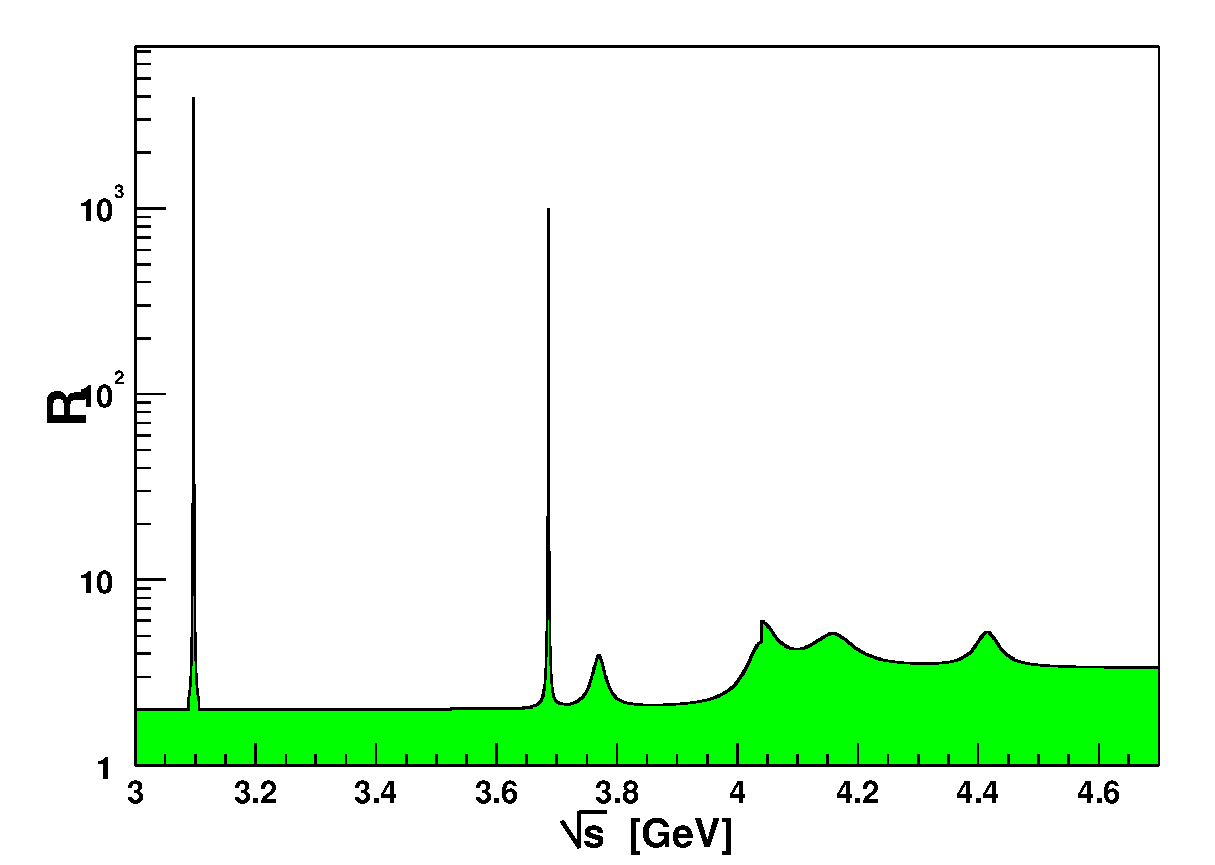
\epsfig{file=cRpsi.eps,width=52mm}

\begin{minipage}{52mm}
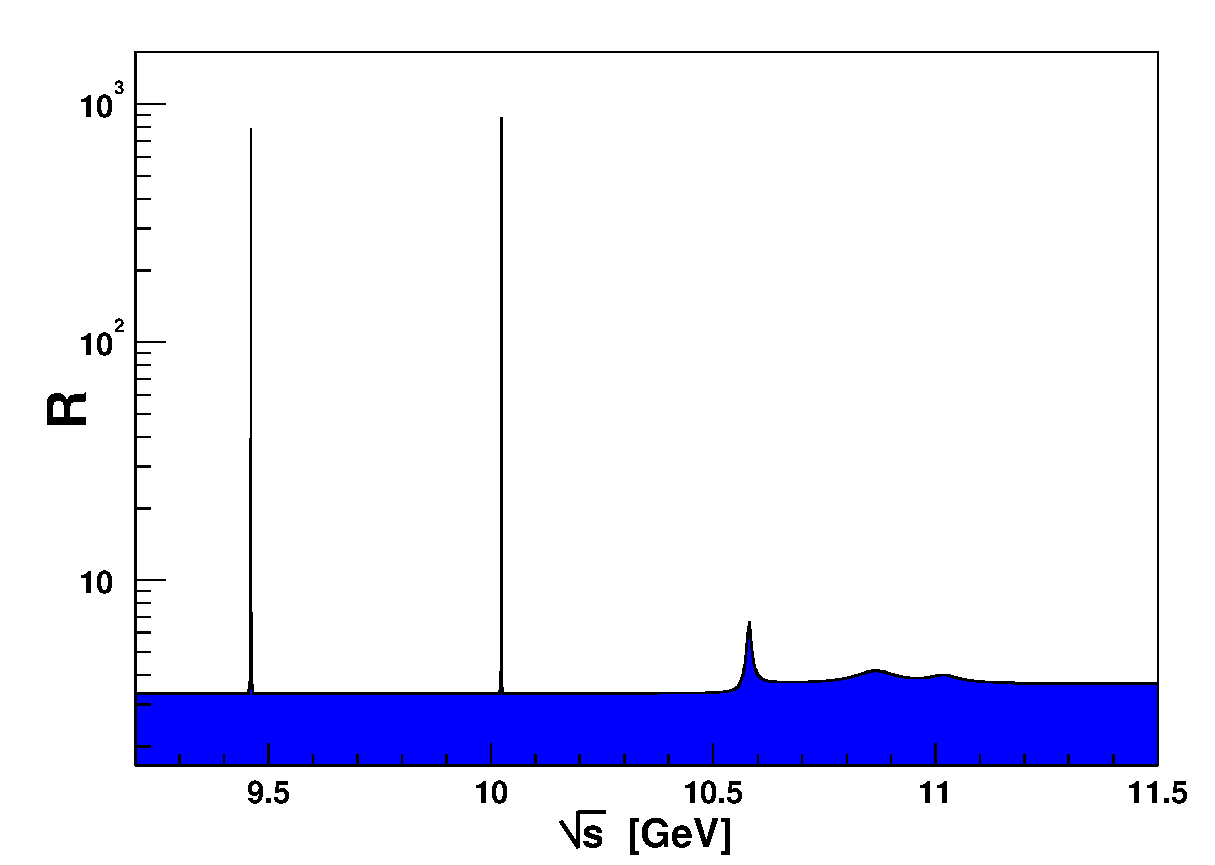
\epsfig{file=cRups.eps,width=52mm}
\end{minipage}
\begin{minipage}{52mm}
\small\bf
This hadronic experimental distribution $R(s)$ is now implemented in package RRes by M. Boonekamp
and used in \KK MC for low $Q^2$ quark-pair spectrum
\end{minipage}

\vfill
\end{slide}    %%%
%%%%%%%%%%%%%%%%%%


%//////////////////////////////////////////////////////////////////////////////////
%//////////////////////////////////////////////////////////////////////////////////
\begin{slide}
\yellowbox{\crd\bf Split of continuum into channels}
\begin{center}
  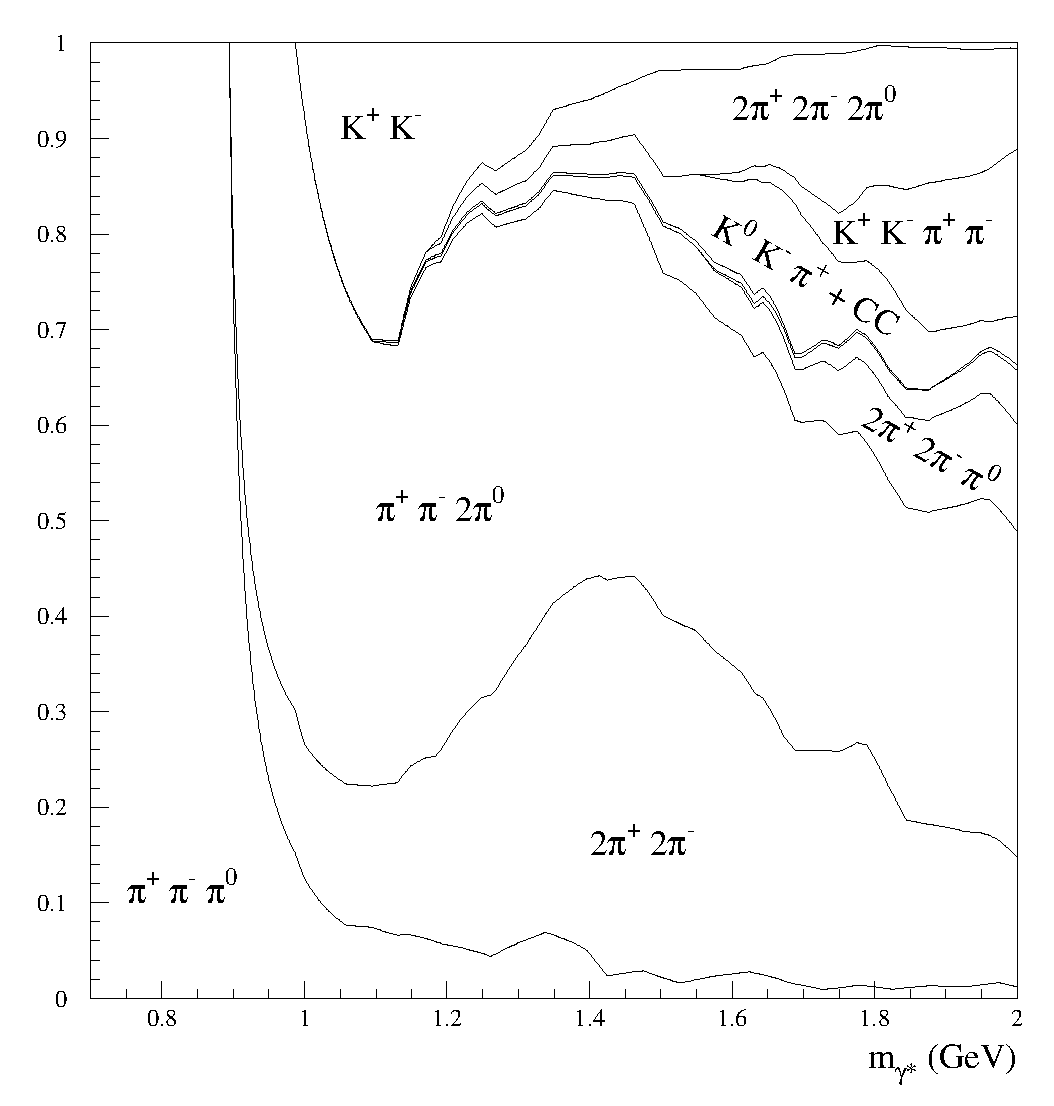
\epsfig{file=BRg.eps,width=80mm,height=60mm}
\end{center}

\small\bf
Experimental data are used to determine channel in the non-resonant part below 2GeV.

\vfill
\end{slide}    %%%
%%%%%%%%%%%%%%%%%%


%//////////////////////////////////////////////////////////////////////////////////
%//////////////////////////////////////////////////////////////////////////////////
%\begin{slide}
%\yellowbox{\bf\crd  Radiative return at KLOE, as seen with \KK MC. PRELIMINARY! }
%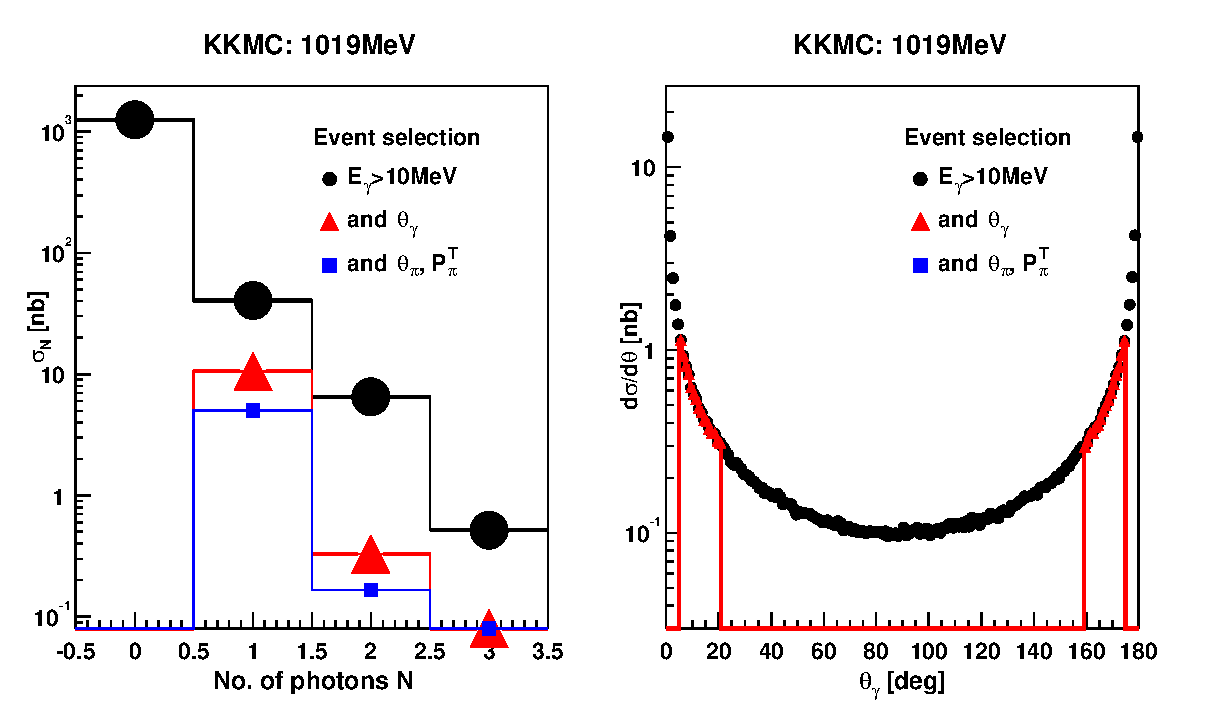
\epsfig{file=../Plots/cFig1.eps,width=57mm}
%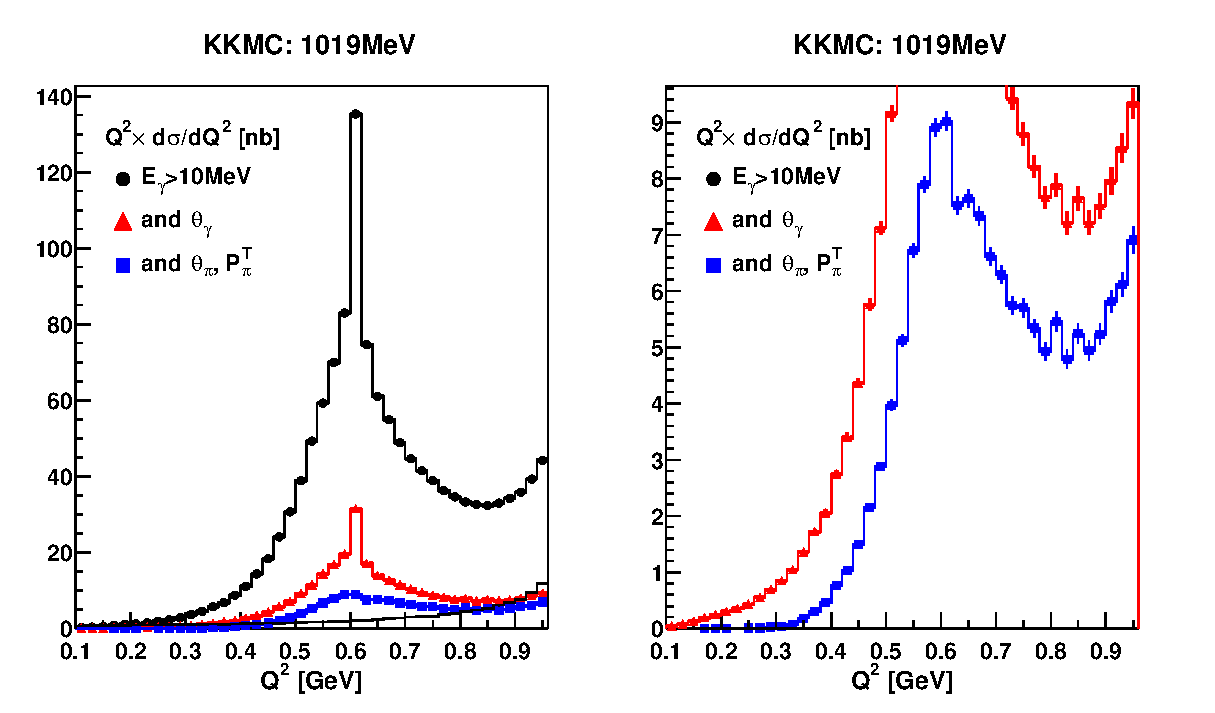
\epsfig{file=../Plots/cFig2.eps,width=57mm}
%Event selection as in KLOE paper hep-ex/0106100:\\
%$ 5^\circ <\Theta_\gamma< 21^\circ,\quad  159^\circ <\Theta_\gamma< 175^\circ,\quad E_\gamma>10MeV $\\
%$ 55^\circ <\Theta_\pi< 125^\circ,\quad p_\pi^T>200MeV$.
%\vfill
%\end{slide}    %%%
%%%%%%%%%%%%%%%%%%


%//////////////////////////////////////////////////////////////////////////////////
%//////////////////////////////////////////////////////////////////////////////////
\begin{slide}
\yellowbox{\bf\crd  Radiative return at KLOE with \KK MC. PHOTON DISTRIBUTIONS }
\vspace{-3mm}
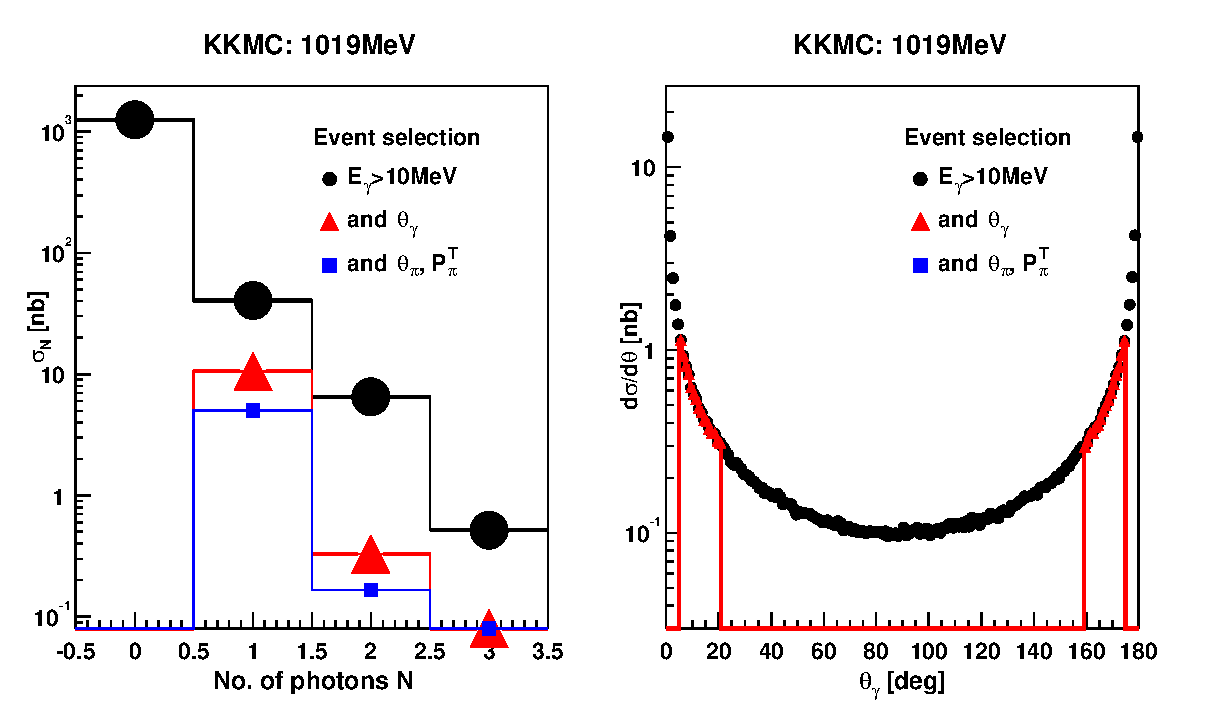
\epsfig{file=../Plots/cFig1.eps,width=100mm}
\\
Event selection as in KLOE paper hep-ex/0106100:\\
$ 5^\circ <\Theta_\gamma< 21^\circ,\quad  159^\circ <\Theta_\gamma< 175^\circ,\quad E_\gamma>10MeV $\\
$ 55^\circ <\Theta_\pi< 125^\circ,\quad p_\pi^T>200MeV$.\\
N.B. TWO photons within the ``detection window'' with $\sim 3\%$ probability!
\vfill
\end{slide}    %%%
%%%%%%%%%%%%%%%%%%


%//////////////////////////////////////////////////////////////////////////////////
%//////////////////////////////////////////////////////////////////////////////////
\begin{slide}
\yellowbox{\bf\crd  Radiative return at KLOE with \KK MC. $Q^2_{\pi^+\pi^-}$ DISTRIBUTIONS }
\vspace{-3mm}
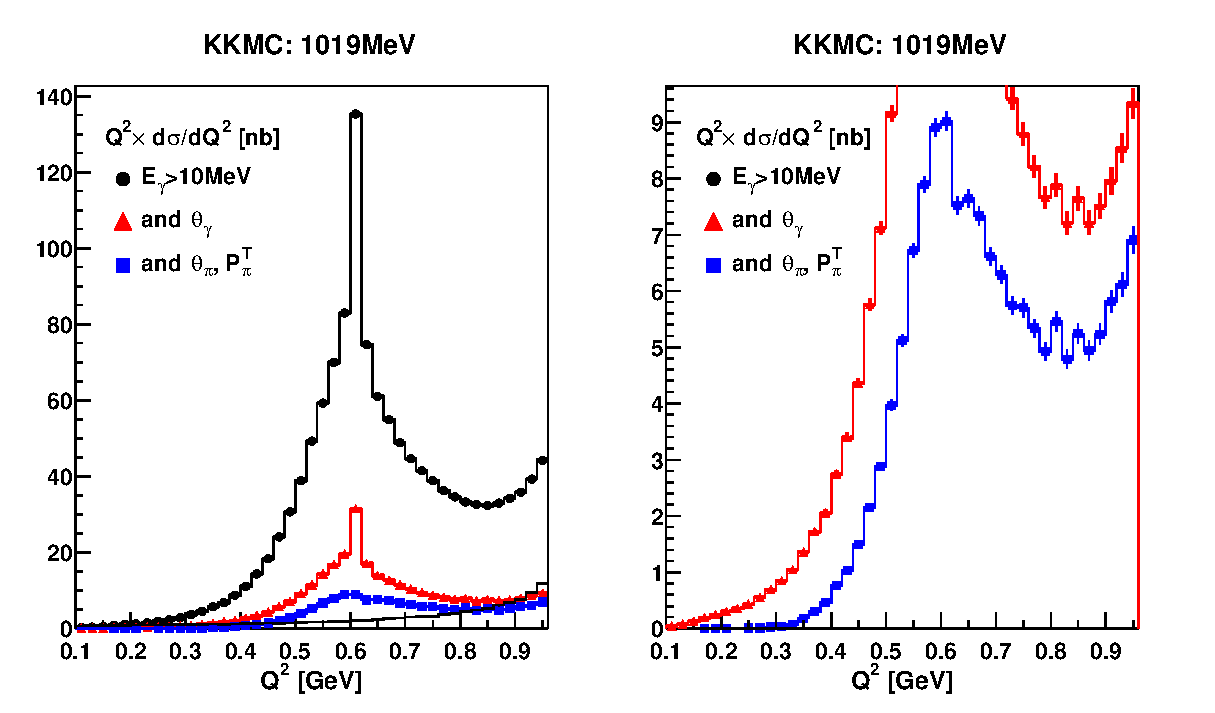
\epsfig{file=../Plots/cFig2.eps,width=100mm}
\\
Event selection as in KLOE paper hep-ex/0106100:\\
$ 5^\circ <\Theta_\gamma< 21^\circ,\quad  159^\circ <\Theta_\gamma< 175^\circ,\quad E_\gamma>10MeV $\\
$ 55^\circ <\Theta_\pi< 125^\circ,\quad p_\pi^T>200MeV$.\\
CEEX \Order{\alpha^2} matrix element.
\vfill
\end{slide}    %%%
%%%%%%%%%%%%%%%%%%


%//////////////////////////////////////////////////////////////////////////////////
%//////////////////////////////////////////////////////////////////////////////////
\begin{slide}
%\yellowbox{\bf\crd  KKMC versus PHOKARA }
\vspace{-3mm}
{\footnotesize
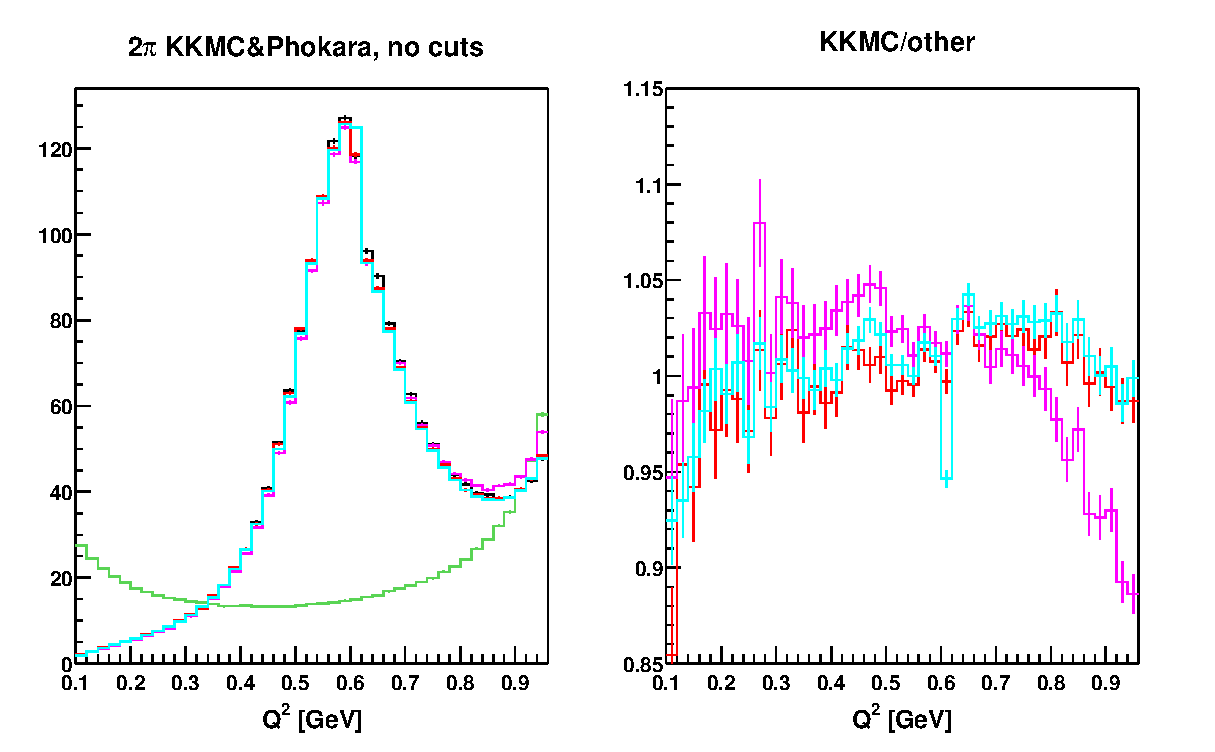
\epsfig{file=../Plots/cFig2c1.eps,width=100mm}
  ds\_dqq\_phokhara\_g\_10e6\_born\_0\_180\_0\_180.dat {\cmg MAGENTA} \\
  ds\_dqq\_phokhara\_g\_10e6\_nlo\_0\_180\_0\_180.dat~~  {\red RED} \\
  KKMC {\bf BLACK}, ~~~~~~~~Muon pair KKMC {\cgr GREEN}, ~~~~~~~~Axel, CYAN\\
  Note:  No cut on pions! For KKMC $\pi^+\pi^-$ from $\phi$ is NOT excluded.
}
\vfill
\end{slide}    %%%
%%%%%%%%%%%%%%%%%%


%//////////////////////////////////////////////////////////////////////////////////
%//////////////////////////////////////////////////////////////////////////////////
\begin{slide}
%\yellowbox{\bf\crd  KKMC versus PHOKARA  }
\vspace{-3mm}
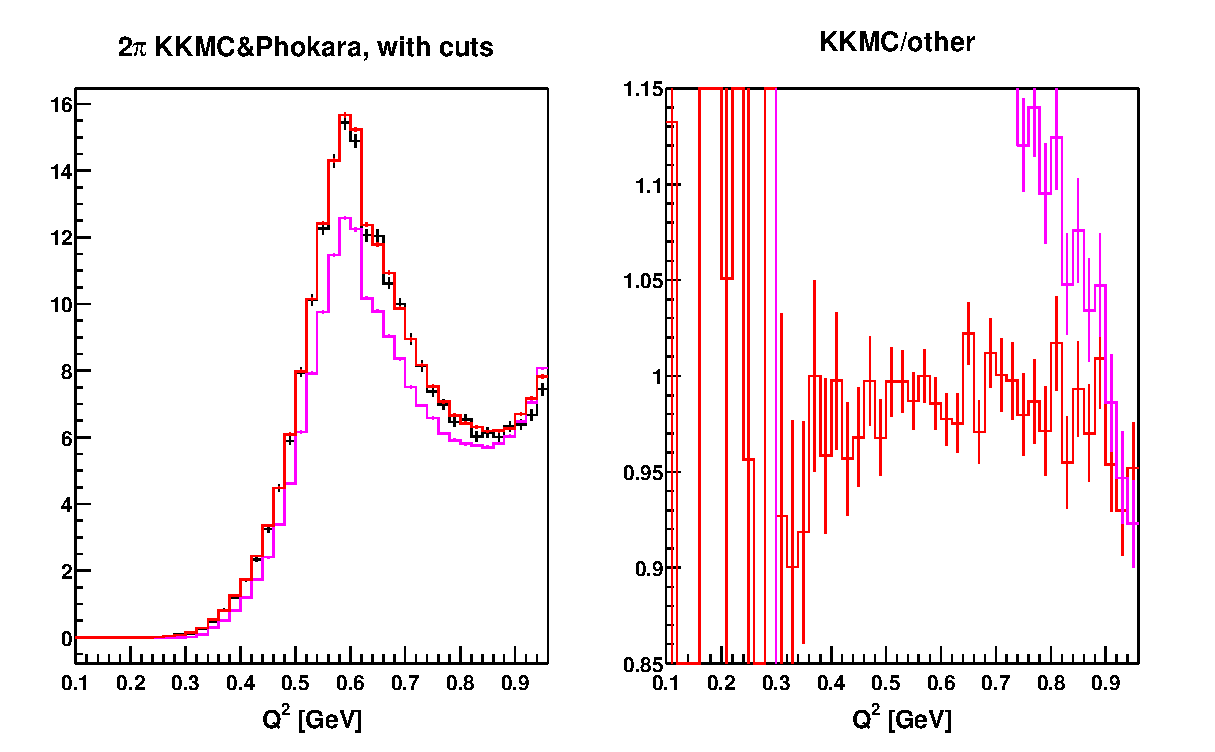
\epsfig{file=../Plots/cFig2c2.eps,width=100mm}
{\footnotesize
  $5^\circ<\vartheta_\gamma <21^\circ $ and $55^\circ<\vartheta_{\pi_{\pm}} <125^\circ $\\
  ds\_dqq\_phokhara\_g\_10e6\_born\_5\_21\_55\_125.dat  {\cmg MAGENTA}, \\
  ds\_dqq\_phokhara\_g\_10e6\_nlo\_5\_21\_55\_125.dat   {\crd RED},\\
  KKMC {\bf BLACK},~~~~~~~~~~~~~
  Note1: for KKMC cut on ``explicit photon'', not on missing energy momentum!\\
  Note2: for KKMC also $p^T_\pi>200MeV$ cut and $\pi^+\pi^-$ from $\phi$ is not excluded!
}
\vfill
\end{slide}    %%%
%%%%%%%%%%%%%%%%%%



%//////////////////////////////////////////////////////////////////////////////////
%//////////////////////////////////////////////////////////////////////////////////
\begin{slide}
\yellowbox{\bf\crd  extra tests, unfinished }
\vspace{-3mm}
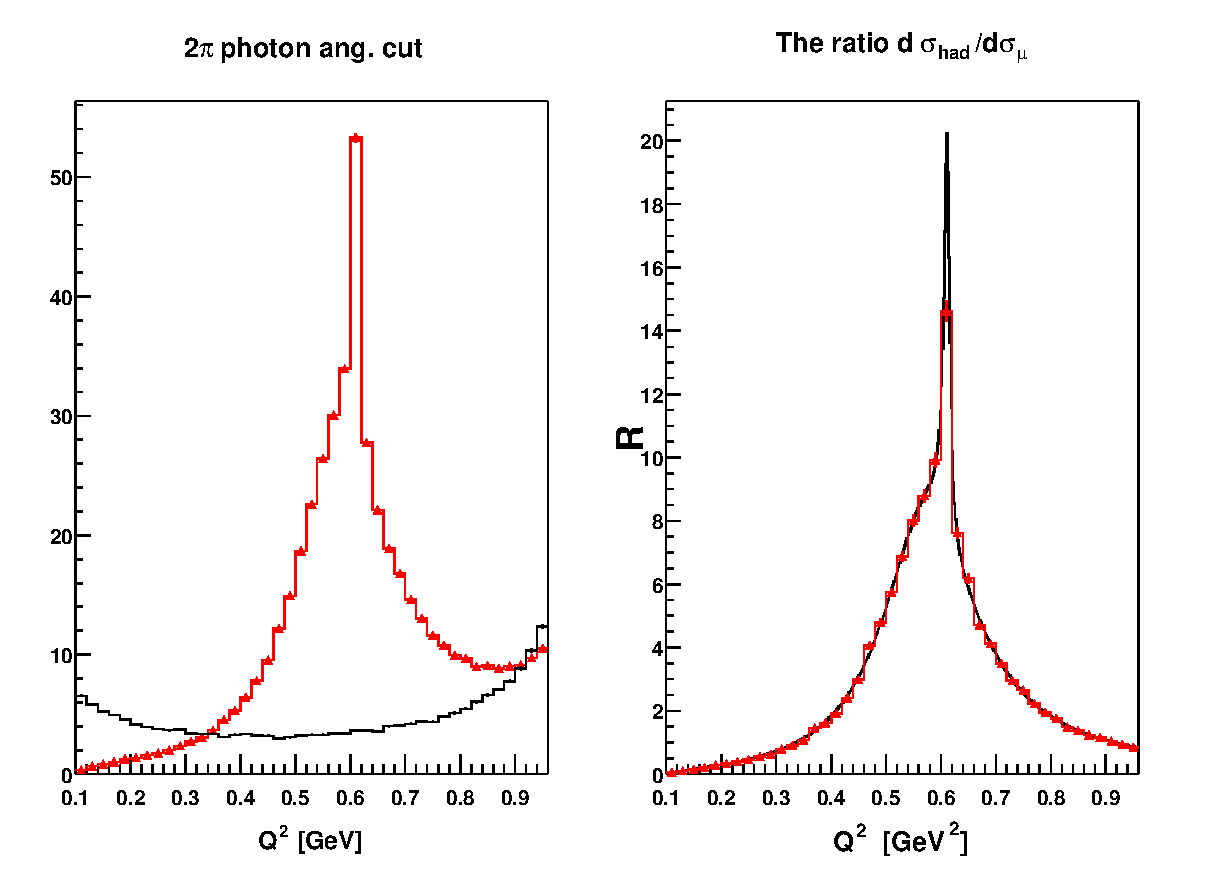
\epsfig{file=../Plots/cFig2b2.eps,width=50mm}
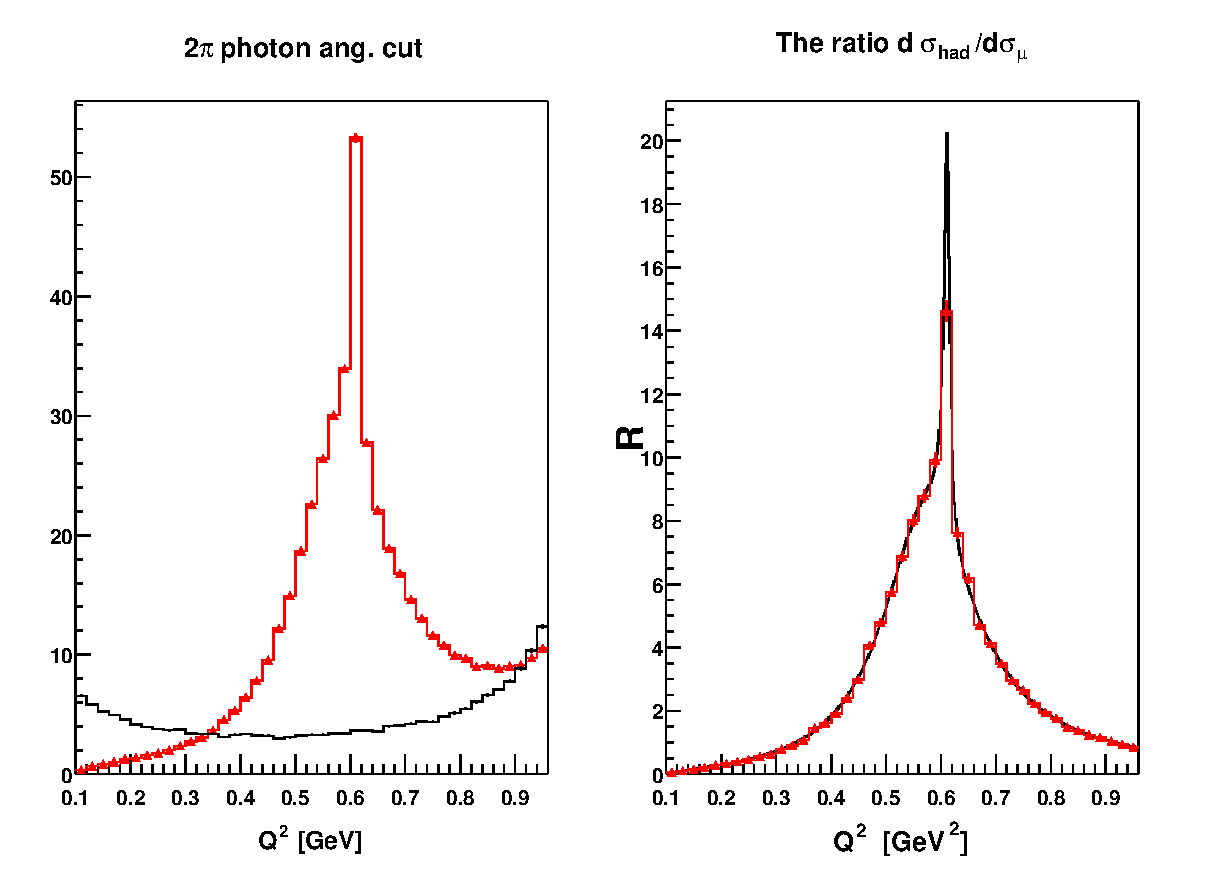
\epsfig{file=../Plots/cFig2b2.eps,width=50mm}
\\
\vfill
\end{slide}    %%%
%%%%%%%%%%%%%%%%%%


%//////////////////////////////////////////////////////////////////////////////////
%//////////////////////////////////////////////////////////////////////////////////
\begin{slide}
%\yellowbox{\bf\crd  KKMC LLexp versus PHOKARA Born and NLO}
\vspace{-3mm}
\begin{center}
  \epsfig{file=../Plots/cFig3a1.eps.EEX.244M,height=60mm,width=120mm}
\end{center}
\vspace{-2mm}
{\footnotesize\bf
  phokara\_born\_1\_qq.dat~~ {\cmg BORN MAGENTA} \\
  phokara\_nlo\_1\_qq.dat~~  {\red NLO RED} \\
  KKMC {\bf BLACK}, ~~~~~~~~Muon pair KKMC {\cgr GREEN},\\
  NOTES:  No cut on pions nor photons!
  Now KKMC and Phokhara are run at the same CMS energy.
  (For KKMC $\pi^+\pi^-$ from $\phi$ is excluded).
}
\vfill
\end{slide}    %%%
%%%%%%%%%%%%%%%%%%



%//////////////////////////////////////////////////////////////////////////////////
%//////////////////////////////////////////////////////////////////////////////////
\begin{slide}
%\yellowbox{\bf\crd  KKMC LLexp versus PHOKARA Born and NLO}
\vspace{-3mm}
\begin{center}
  \epsfig{file=../Plots/cFig3a2.eps.EEX.244M,height=60mm,width=120mm}
\end{center}
\vspace{-2mm}
{\footnotesize\bf
  phokara\_born\_2\_qq.dat~~ {\cmg BORN MAGENTA} \\
  phokara\_nlo\_2\_qq.dat~~  {\red NLO RED},~~~~~ KKMC {\bf BLACK},\\  
  With cuts:~~~ $\vartheta_\gamma<15^\circ$, ~~~~
  $E_\gamma>10$MeV,~~~~
  $ 40^\circ <\vartheta_\pi< 140^\circ$,~~~~
  $p^T_\pi > 0.2$GeV.\\
  The $p^T_\pi$ cut not included in Pkokara results.
  KKMC run at slightly off-resonance 1.02100GeV.
}
\vfill
\end{slide}    %%%
%%%%%%%%%%%%%%%%%%



%//////////////////////////////////////////////////////////////////////////////////
%//////////////////////////////////////////////////////////////////////////////////
\begin{slide}
\yellowbox{\bf\crd  KKMC CEEX versus KKsem, muons, 14apr 8AM}
\vspace{-3mm}
\begin{center}
  \epsfig{file=../Plots/cFig3b1.eps.MuCEEX.32M,height=60mm,width=120mm}
\end{center}
\vspace{-2mm}
{\footnotesize\bf
  Muon pairs.
  KKMC {\crd CEEX} versus KKsem, the best NLL+LL3 exponentiated analytical ISR.
  (Corrected error in Born of KKsem).
}
\vfill
\end{slide}    %%%
%%%%%%%%%%%%%%%%%%


%//////////////////////////////////////////////////////////////////////////////////
%//////////////////////////////////////////////////////////////////////////////////
\begin{slide}
\yellowbox{\bf\crd  KKMC CEEX versus KKsem and Phokhara, muons, 14apr 8AM}
\vspace{-3mm}
\begin{center}
  \epsfig{file=../Plots/cFig3b1.eps.MuCEEX.30M,height=60mm,width=120mm}
\end{center}
\vspace{-2mm}
{\footnotesize\bf
  Muon pairs.
  KKMC {\crd CEEX} versus KKsem, the best NLL+LL3 exponentiated analytical ISR.
  (Corrected error in Born of KKsem).
}
\vfill
\end{slide}    %%%
%%%%%%%%%%%%%%%%%%


%//////////////////////////////////////////////////////////////////////////////////
%//////////////////////////////////////////////////////////////////////////////////
\begin{slide}
\yellowbox{\bf\crd  KKMC EEX versus KKsem, muons}
\vspace{-3mm}
\begin{center}
  \epsfig{file=../Plots/cFig3b1.eps.EEX.244M,height=60mm,width=120mm}
\end{center}
\vspace{-2mm}
{\footnotesize\bf
  Muon pairs.
  {\cgr KKMC EEX} versus KKsem with the best NLL+LL3 exponentiated analytical ISR.\\
  {\crd Phokhara NLL} versus KKsem 
  (lack of exponentiation in Phokhara is $<1\%$).\\
  Finally we plot ratio {\cmg KKMC.EEX/Phokhara.NLL} which
  features (i) incomplete NLO in KKMC.EEX (low $Q^2$)
  and (ii) lack of exponentiation in Phokhara (high $Q^2$).
}
\vfill
\end{slide}    %%%
%%%%%%%%%%%%%%%%%%


%//////////////////////////////////////////////////////////////////////////////////
%//////////////////////////////////////////////////////////////////////////////////
\begin{slide}
%\yellowbox{\bf\crd  KKMC EEX versus KKsem, pions}
\vspace{-3mm}
\begin{center}
  \epsfig{file=../Plots/cFig3b2.eps.EEX.244M,height=60mm,width=120mm}
\end{center}
\vspace{-2mm}
{\footnotesize\bf
  KKMC {\crd EEX} versus KKsem with the best NLL2+LL3 exponentiated analytical ISR.\\
  Phi chanel included both in in KKsem and in KKMC!
  (This is because it is easier to include2 phi in KKsem)
}
\vfill
\end{slide}    %%%
%%%%%%%%%%%%%%%%%%


%//////////////////////////////////////////////////////////////////////////////////
%//////////////////////////////////////////////////////////////////////////////////
\begin{slide}
\yellowbox{\bf\crd Conclusions }

{\bf\cbl
  \begin{itemize}
  \item
    KKMC.CEEX and KKsem (LL3 + NLO) agree very well, in entire $Q^2$ range.
  \item
    KKMC.EEX lacks NLO $1\%$ at $Q^2=0.5$GeV$^2$ and up to $3\%$ at low $Q^2$,
    see ratio KKMC.EEX/KKsem.\\
    Most probably $3\%$ is technical artefact and
    the effect is much smaller. Work in progress!
  \item
    Phokhara NLO lacks LL3 and exponentiation: 
    about $<<1\%$ at $Q^2=0.5$GeV$^2$ and up to $1\%$ at high $Q^2$.
    see ratio Phokhara.NLO/KKsem.
    This effect is reproduced by KKsem very precisely.
  \item
    Most probably we shall end up with the ratio KKMC.EEX/Phokhara.NLO 
    $<<1\%$ for entire $Q^2$ range.
    $3\%$ at low $Q^2$ has to be debugged.
  \end{itemize}
}

\vfill
\end{slide}    %%%
%%%%%%%%%%%%%%%%%%


\end{document}                                           %%%%%%%%%%%%%%%%%%%%
%%%%%%%%%%%%%%%%%%%%%%%%%%%%%%%%%%%%%%%%%%%%%%%%%%%%%%%%%%%%%%%%%%%%%%%%%%%%%
%%%%%%%%%%%%%%%%%%%%%%%%%%%%%%%%%%%%%%%%%%%%%%%%%%%%%%%%%%%%%%%%%%%%%%%%%%%%%

